%%
%% This is file `sample-sigconf.tex',
%% generated with the docstrip utility.
%%
%% The original source files were:
%%
%% samples.dtx  (with options: `sigconf')
%% 
%% IMPORTANT NOTICE:
%% 
%% For the copyright see the source file.
%% 
%% Any modified versions of this file must be renamed
%% with new filenames distinct from sample-sigconf.tex.
%% 
%% For distribution of the original source see the terms
%% for copying and modification in the file samples.dtx.
%% 
%% This generated file may be distributed as long as the
%% original source files, as listed above, are part of the
%% same distribution. (The sources need not necessarily be
%% in the same archive or directory.)
%%
%% The first command in your LaTeX source must be the \documentclass command.
\documentclass[sigconf, nonacm, natbib, screen, balance=False]{acmart}

% Documentation for packages
% - ACM Article Template
%    https://www.acm.org/publications/proceedings-template
% - Pseudocode typesetting CLRS-style:
%    https://www.cs.dartmouth.edu/~thc/clrscode/clrscode3e.pdf
% - Python code typesetting
%    http://ctan.uib.no/macros/latex/contrib/listings/listings.pdf
% - AMS Math
%    http://ctan.uib.no/macros/latex/required/amsmath/amsldoc.pdf
% - Graphics
%    http://ctan.uib.no/macros/latex/required/graphics/grfguide.pdf

\usepackage{makecell}
\renewcommand\theadalign{bc}
\renewcommand\theadfont{\bfseries}
\renewcommand\theadgape{\Gape[0pt]}
\renewcommand\cellgape{\Gape[0pt]}

\usepackage[colorinlistoftodos]{todonotes}
%\usepackage[disable]{todonotes}
\usepackage{clrscode3e}  
\usepackage{listings}
\lstset{language=Python, basicstyle=\ttfamily}

% based on https://tex.stackexchange.com/questions/279240/float-for-lstlisting
\usepackage{float}
\floatstyle{ruled}
\newfloat{listing}{tbph}{lop}
\floatname{listing}{Listing}
\def\lstfloatautorefname{Listing} % needed for hyperref/auroref

\citestyle{acmauthoryear}
\settopmatter{printfolios=true}  % show page numbers

%% end of the preamble, start of the body of the document source.
\begin{document}

%%
%% The "title" command has an optional parameter,
%% allowing the author to define a "short title" to be used in page headers.
\title{Spring Wheat Yield prediction based on UAV Imagery}
\subtitle{Data Science Report, NMBU, Spring 2021}

\author{Muhammad Fahad Ijaz}
\email{muhammad.fahad.ijaz@nmbu.no}

%% The abstract is a short summary of the work to be presented in the
%% article.
\begin{abstract}
  This report is a part of vPheno (virtual phenotyping) project at NMBU that started in 2017. The aim of the project is to reduce the time it takes to develop more robust cultivars. So, using the data that has been collected as part of this project from 2017, I tried to develop machine learning models to predict the grain yield of spring wheat, using the data extracted from the images taken by Unmanned Aerial Vehicles (UAVs). The features extracted from the images were fed into the machine learning algorithm that predicted the yield. The results are discussed, and suggestion are included to improve the data collection methods and, consequently, the results for future studies.
\end{abstract}
\todo{check all reference have Text 'Table' where cited in text}


%%
%% This command processes the author and affiliation and title
%% information and builds the first part of the formatted document.
\maketitle

\section{Introduction}\label{sec:intro}

The world population is increasing rapidly \todo{ref??} and so is the global food demand. Wheat is the most important food source all around the world \cite{Igrejas2020}. The global demand for wheat is projected to more than double by the year 2050 \cite{tilman}. This stresses the need for the increase in yield of food crops.
\todo{connect the sentences in the paragraph following. Hans}
There are several methods for increasing the yield of wheat. The most common and traditional is based on the yield of the crop.\todo{Are there other methods? give a ref to the brfeeding practices}
 The crop is cultivated, yield is calculated which is used to make decision if that crop is to be used for breeding or not. This is a very time-consuming process\todo{Can you give numbers for how long this takes, both for a single experiment and for actually developing an improved strain?} and involves a substantial cost as well. In this fast pace innovation age, there is a high demand to speed up the processes that can improve yield. \todo{"fast pace innovation age" is dangerously close to "blurb" that may fit in marketing brochures but not in scientific reports. Furthermore, as you point out above, the motivation to speed up wheat development is not to keep up with the speed of innovation in Silicon Valley, but plain and simple to have a chance to feed the world.}


Remote sensing systems can be deployed to get the information in real time and then the data collected can be used to predict the yield. One such technique is to deploy Unmanned Aerial Vehicles (UAVs) to gather data from the field. That data is used to then predict different characteristics of the plants. Those traits include grain yield as well. My goal is to develop a model which can predict the yield of the crop with greater accuracy.\todo{redefine goal}


\subsection{Problem Definition}\label{sec:problem_def}

Since the cultivated land is limited and it costs a lot to convert barren land to cultivable, the better approach would be to focus on increasing the yield from the existing cultivable land. Moreover, cultivating more land would naturally cost more than cultivating less land and getting more production. So, the reason and motivation behind plants phenotyping is to increase the yield from the same fields. Regular phenotyping approached are slow and costly. Using remote sensing for this can be fast and cheap. That is the motivation behind the vPheno project at NMBU that aims at reducing the time?? required to experiment with different varieties of wheat and enable them to do accurate selection of potential varieties of wheat. Machine learning algorithms will be used for this purpose.
This report contributes to the research project vPheno (virtual phenomics) at the Faculty of Bioscience at NMBU. The project, started in 2017, aims to help plant breeders reduce the time required to select better, high yield varieties of crops and speedup the process using image analysis techniques. There have been a few studies at NMBU by \citet{burud_bleken}, \citet{grindbakken} and \citet{lied}. This report explores a different way of combining data, collected for different fields at different occasions. Moreover, including data for the year 2019 as input as well that has recently become available.\todo{Include 2020 data as well, probably or just use robot.}


The objective of this report is to generate a machine learning model that can predict the grain yield of wheat based on the image data collected from the field at different times during the season.
\todo{After this paragraph, provide a brief overview over the paper: what is in which section?}


\section{Theory}\label{sec:theory}

\subsection{Plant Phenotyping}\label{sec:plant_pheno}

Plant phenotyping is the study of how traits of the plants, termed as phenome, develop from their interaction with the environment and how their genome can be related to those traits \cite{minervini}. These traits include, among others, the plant yield, maturity time, plant height, etc. The importance of phenotyping has increased significantly with the increased demand for improving the yield.
Plant phenotyping investigates how a plant's genome affects the observable traits of a plant (phenome). It is becoming increasingly important in our quest towards efficient and sustainable agriculture. While sequencing the genome is becoming increasingly efficient, acquiring phenotype information has remained of low throughput. 
Image based phenotyping are fast and nondestructive. They can predict the results and save time to make decision about the choice of the variety of wheat to be chosen for the next phase

\subsection{Spectral Indices}\label{sec:aspect1}

Spectral indices are derived values from one or more reflection bands. The are several different spectral indices. The ones related to plants are called vegetation indices. We are focusing on the ones that can be derived from the spectral bands data we have for the project. The relevant vegetation indices and the formula to calculate them are as follows.

	The MERIS terrestrial chlorophyll index – MTCI
\begin{displaymath}
  \caption{MTCI Equation}
  \label{eq:mtci}
MTCI=\ \ \frac{NIR-RedEdge}{RedEdge-Red}
\end{displaymath}
  \caption{MTCI Equation}

	Normalized difference vegetation index – NDVI
\begin{displaymath}
  \caption{NDVI Equation}
  \label{eq:ndvi}
NDVI=\ \frac{NIR-RED}{NIR+RED}
\end{displaymath}

	Enhanced vegetation index - EVI
\begin{displaymath}
  \caption{EVI Equation}
  \label{eq:evi}
EVI=\ 2.5\ \times\frac{NIR-RED}{NIR+(6\times R E D)-(7.5\times B L U E)+1}
\end{displaymath}


\section{Method}\label{sec:theory}

\subsection{Process Overview}\label{sec:aspect1}

The data is collected from three fields where spring wheat has been planted. Data collection is done by using a UAV equipped with an RGB Camera, in addition to a multispectral camera, GPS Module and an ambient light sensor. The UAV is flown over the field on a predefined grid pattern path and collected the image data. The image data is then stitched to get an overall image of the field. This is done using Pix4D Software \cite{lied}. The data collected by the system consists of blue, green, red, red edge and near-infrared bands. Normalized Difference Vegetation Index (NDVI), MERIS Terrestrial Chlorophyll Index (MTCI), and Enhanced Vegetation Index (EVI) are calculated using the bands data.

\subsection{Test Site}\label{sec:aspect1}

The test site is located at Vollebekk Research Farm, close to NMBU in Ås. The coordinates of the site are 59°39'23.6"N 10°45'13.8"E. For this study, one spring wheat field is included. The field is further subdivided into small subplots. Different candidate cultivars are cultivated in the plots with each cultivar usually being planted in two sub plots. The placement of the cultivars is random with randomization being done in an alpha-lattice design. 


\begin{table}[h!]
  % Table captions always come *above* the table.
  \caption{Details of field where the data has been collected from}
  \label{tab:fields}
  \begin{tabular}{lll}
    \hline
    Name of Field & Details & Season\\Sowing Date \\\hline
    \verb!Robot! & \verb!Historical Cultivars! & \verb!10th May, 2018! \\
  \end{tabular}
\end{table}


\begin{figure}[h]
  \centering
   \hspace*{-0.25in}
   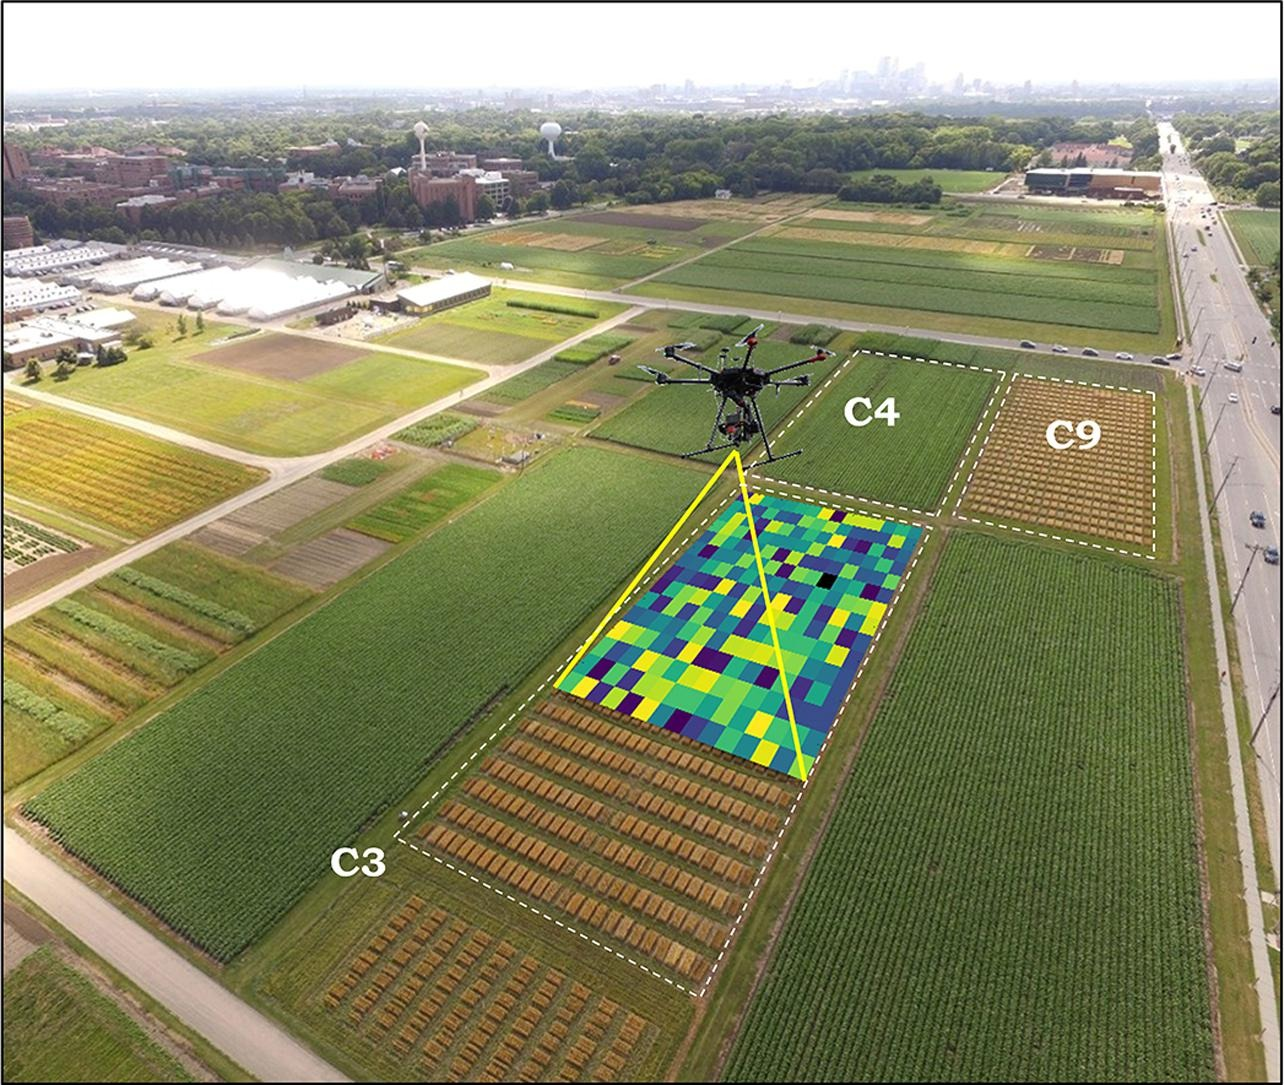
\includegraphics[width=0.4\textwidth, angle=0,]{moghimi.jpg}
  % figure captions below figure
  \caption{A demonstration of the data collection process \cite{moghimi}}
  %% Explain the size of the data used

  \label{fig:example}
\end{figure}


Each subplot is separated from the neighboring subplots by a border row. This is done to reduce the border effect. As a standard agronomic practice, herbicides and fungicides are used on the crops to ensure better yield. In addition to the image data, manual measurements are also being done to calculate the number of days to maturity and number of days to heading of the plant. Plant height is also measured once before harvest, when the plants are at their maximum growth height. Grain yield is measured in gram/m^2.

\subsection{Image Data Collection}\label{sec:aspect1}

The image data is collected by a UAV which had been mounted with necessary equipment to gather the image and multispectral data. The UAV used is DJI Phantom 4. It comes with a GPS Module and an RGB Camera which are used to gather the RGB image data. In addition to that, a RedEdge Downwelling Light Sensor (DLS) \cite{light_sensors:online} from Micasense and a RedEdge-M multispectral by Micasense \cite{RedEdgeM:online} are used as well \cite{lied}. The image resolution of the RGB camera is 3000x4000 pixels. 
The lighting conditions vary a lot from season to season and weather. This affects the consistency of the collected data. This effect needs to be compensated for to get reliable data in the long run. The ambient light sensors are used to compensate for that \cite{Bestpractices_mica:online}.
The data collected by the multispectral camera in 5 bands, is listed in table \ref{tab:bands}.


\begin{table}[h!]
  % Table captions always come *above* the table.
  \caption{Table with details of bands data collected by the multispectral camera \cite{RedEdgeM:online} \cite{lied}}
  \label{tab:bands}
  \begin{tabular}{lll}
    \hline
    Band Name & Center wavelength (nm) & Bandwidth (nm) \\\hline
    \verb!Blue! & \verb!475! & \verb!20! \\
    \verb!Green! & \verb!560! & \verb!20! 
    \verb!Red! & \verb!668! & \verb!10! 
    \verb!REG! & \verb!717! & \verb!10! 
    \verb!NIR! & \verb!840! & \verb!40! 

  \end{tabular}
\end{table}




\subsection{Images Stitching}\label{sec:aspect1}

After the images are collected using the equipment described, the next step is to stitch them together to form one big image of the field. This is done in Pix4D. This is detailed in \cite{lied}.

\subsection{Data Extraction}\label{sec:aspect1}

QGIS application is used to extract the required data from the reflectance map generated from the data collected from the cameras on the UAV. QGIS is an open-source Geographical Information System, commonly referred to as GIS. Geoprocessing, sampling, geometry, and vector analysis are some of the applications of QGIS. In this case, a custom grid is generated using QGIS matching the setup of subplots in the field \cite{lied}. Next, it extracts the required values of the bands for each subplot from the grid. This data is exported to an Excel sheet. 

\subsection{Detail of available data}\label{sec:aspect1}


In table \ref{tab:robot} are the details of the remote sensing datasets available for the robot field from 2017, 2018 and 2019. The datasets taken at different dates have varying number of features. For, examples, the 2017 data does not have the blue band because at the time of data collection, the equipment lacked the capability to capture the blue band. So, in those datasets, the blue band data is not available. Since EVI calculations require the data from blue band, that is also missing for those datasets. Those datasets are not used for that reason. Only the available data from 2018 and 2019 is used since they have the required input variables to be used for training the machine learning model.
The details of the datasets is given in the table \ref{tab:robot}.




\begin{table}[h!]
  % Table captions always come *above* the table.
  \caption{Remote sensing data Robot Field}
  \label{tab:robot}
  \begin{tabular}{|c|c|c|c|c|}
    \hline
    %Robot & \multicolumn{3}{c|}
    Field & Year & Dates & Samples & Comments \\
    \hline
    %\multirow {7}{*}{\makecell{Blue band\\ \& EVI missing}}
    
     &  & 14/06/2017 & 96 & \\
    \cline{3-4}
     &  & 19/06/2017 & 96 &\\
    \cline{3-4}
     &  & 29/06/2017 & 96 & \\
    \cline{3-4}
     & 2017 & 03/07/2017 & 96 & \makecell{Blue band}\\
    \cline{3-4}
    Robot &  & 14/07/2017 & 96 &  \makecell{\& EVI missing}\\
    \cline{3-4}
     &  & 17/07/2017 & 96 & \\
    \cline{3-4}
     &  & 14/08/2017 & 96 & \\
    \cline{2-5}
     &  & 02/07/2018 & 96 & \\
    \cline{3-4}
     &  & 05/07/2018 & 96 & \\
    \cline{3-4}
     & 2018 & 11/07/2018 & 96 & Complete\\
    \cline{3-4}
     &  & 19/07/2018 & 96 & \\
    \cline{3-4}
     &  & 24/07/2018 & 96 & \\
    \hline

  \end{tabular}
\end{table}


This summary is given in table \ref{tab:summary}
It summarizes the data being selected for further processing.


\begin{table}[h!]
  % Table captions always come *above* the table.
  \caption{Summary of status of data }
  \label{tab:summary}
  \begin{tabular}{lll}
    \hline
    Year & Data samples & Details\\\hline
    \verb!2017! & \verb!96! & \verb!Blue band missing! \\
    \verb!2018! & \verb!96! & \verb!Complete! 


  \end{tabular}
\end{table}



\subsection{Data Processing}\label{sec:aspect1}
\subsubsection{Target variable and input variable}\label{sec:aspect1}

In the table \ref{tab:bands_detail}, the input variables are listed which are extracted from the image data. In addition to those, there are a few vegetation indices that can be calculated from the bands data. While the age of the crop at the time of data collection is collected manually, i.e., the number of days since the crop was sown. And number of days to maturity.

\begin{table}[h!]
  % Table captions always come *above* the table.

  \caption{Input variables}
  \label{tab:bands_detail}
  \begin{tabular}{|c|c|c|c|}
    \hline
	\makecell{Input\\Variable} & Explanation & Selection & Type \\ \hline
	Blue & Blue band & Median & Band Data  \\ 
	\hline
	Green & Green Band & Median & Band Data \\ 
	\hline
	Red & Red Band & Median & Band Data \\ 
	\hline
	Red Edge & \makecell{Red-NIR\\transition zone}  & Median & Band Data \\ 
	\hline
	NIR & Near Infrared & Median & Band Data \\ 
	\hline
	NDVI & \makecell{Normalized Difference\\Vegetation Index} & Median & Vegetation index \\ 
	\hline
	MTCI & \makecell{The MERIS\\terrestrial \\chlorophyll index} & Median & Vegetation index \\ 
	\hline
	EVI & \makecell{Enhanced vegetation\\index} & Median & Vegetation index \\
	\hline
	Age & \makecell{No. of days\\since crop\\was sown} & Days & \makecell{Difference b/w\\sowing data\\and date of\\image collection} \\
	\hline
  \end{tabular}
\end{table}

There are other variables also available from the data. For example, days to maturity and days to heading but these can only be calculated after the crop has been harvested. Since, in a real-world scenario, this data will not be available to the model while making predictions for new data, these were not included in model training.
The grain yield is the target variable, table \ref{tab:target}.

\begin{table}[h!]
  % Table captions always come *above* the table.
  \caption{Target variable}
  \label{tab:target}
  \begin{tabular}{lll}
    \hline
    Target Variable & Explanation & Units\\\hline
    \verb!Grain_yield! & \verb!Grain Yield! & $gram/{m}^2$ \\

  \end{tabular}
\end{table}


\subsection{Data pre-processing}\label{sec:aspect1}

For each band, there is mean, median, and standard deviation of the band data is derived from the images. The median values are used for all bands for predictions since median values are not affected much by outliers. The age is calculated by subtracting the sowing date from the date the data is collected. 

\subsubsection{Data Compilation Strategy}\label{sec:aspect1}

The previous studies on similar data at NMBU have taken a different approach to data compilation for machine learning model. They compiled the data sets by adding the data collected on different dates as new features in the dataset. This resulted in an enormous increase in the number of features in the dataset, but the number of samples remained the same. The reasoning for this strategy was that since for one plot, although the data is being collected several times in one season, but the yield is the same for all of them. So, it is better to add new features to the same samples than to add them as new samples, as that might confuse the model.
I took a different approach by adding the data collected on different dates, as new samples with the same number of features. So, for Robot in 2018, there are 96 sub-plots, so 96 data samples. The data was collected 5 times in 2018 season. So, the total number of samples amounts to 480. \todo{check after processing}

The data for all the dates has been combined into a single dataset with 9 input variables, one target variables and xxxx data samples.
\todo{check after processing}

\subsubsection{Missing data}\label{sec:aspect1}

There were several data field missing. That results in 14 samples being dropped from the dataset. 13 of them were missing grain\_yield while one is missing Red, NDVI, MTCI and EVI values. After dropping 14 samples, 9270 samples are remaining which have been used for predictions.

\subsection{Machine Learning}\label{sec:aspect1}

Python is being used for the purpose of this report. The machine learning algorithms are from Scikit-Learn (0.23.2), XGBoost (version 1.2.1) and TensorFlow (version 2.3.1) libraries. The analysis and predictions have been executed in a Jupyter Notebook with Python version 3.8.5.

\subsubsection{Sampling and data partitioning}\label{sec:aspect1}

The data split into training and validation sets, with 30 percent data held for validation while the rest used for training. The test\_train\_split function from Scikit-Learn is used for making the split. The data is shuffled during the split. The tuned hyperparameters of which are in Table 4.9. For the rest of the hyperparameters, the default values are used.

\begin{table}[h!]
  % Table captions always come *above* the table.
  \caption{Hyperparameters of test\_train\_split}
  \label{tab:hyptts}
  \begin{tabular}{ll}
    \hline
    Hyperparameter & Value \\\hline
    \verb!test_size! & \verb!0.3! \\
    \verb!shuffle! & \verb!True! \\
    \verb!random_state! & \verb!55! \\\hline
  \end{tabular}
\end{table}

\subsubsection{Standardization}\label{sec:aspect1}

The training and validation input variables have been standardized using the StandardScaler from Scikit Learn \cite{stand_scaler:online}. StandardScaler scales the features to unit variance. This improves the predictions results for most of the machine learning estimators. The default values have been used for the hyperparameters for StandardScaler. 

\subsubsection{Machine Learning Models}\label{sec:aspect1}

This problem requires the machine learning models to predict a continuous target. This is makes it a regression problem. So, regression estimators can be used for that purpose. From Scikit learn, Random Forest Regressor is used. In addition, XGBoostRegressor is also used. The hyperparameters of each of them are given in Appendix A.
In addition, a Neural Networks comprising of one input layer, seven hidden layers, and one output layer is used. The activation function 'relu' has been used in all of them while keeping 'normal' kernel\_initializer. The code can be reviewed at the following notebook.

\url{https://github.com/fahadijaz/spring\_wheat\_yield\_prediction/blob/main/03.ml_nn_dnn.ipynb}

\subsubsection{Code Repository}\label{sec:aspect1}

The code used in data pre-processing and further predictions using the machine learning models can be found at the following repository.
\url{https://github.com/fahadijaz/spring\_wheat\_yield\_prediction/}

\section{Results}\label{sec:aspect1}

While running the predictions results, the estimators have been fed with the original data as is, and also have been tested with the standardized data, standardized using the StandardScaler from Scikit Learn. It turns out the RandomForestRegressor and the XGBoostRegressor give better results with the original, non-transformed data. While the Neural Network gave quite better results with the standardized data.

\subsection{Evaluation Results}\label{sec:aspect1}

The results from the estimators are listed in the Table 5.1
\todo{COrrect table}. It is evident that the RandomForestRegressor has the best results in terms of all the scoring parameters included.

\todo{COrrect table}
Table 5.1: Estimators Evaluation Results
Estimator	MAE	MSE	RMSE	R2
RandomForestRegressor	37.03141441	2454.533461	49.54324839	0.83873311
XGBoostRegressor	38.84113664	2717.994515	52.13438899	0.821423285
Neural Network	38.27009791	2570.24969	50.69763003	0.833658735

The results from a previous study on the similar data \cite{lied}, had varying degree of results accuracy with better results on one data set while worse results than in Table 5.1 for two other datasets.\todo{CITE TABLE NUMBER}


\section{Discussion}\label{sec:aspect1}

\subsection{Assessment of model performance}\label{sec:aspect1}

The models performed well, and the evaluation results were close to each other. There were not any major differences between the results. This indicates that the hyperparameters tuning can improve the accuracy to some extent but not by a landslide. More data can help in improving the results, in addition to defining and collecting more features related to the crop, and the conditions surrounding it.

% In the acks section, you can thank people for help.
\begin{acks}
We are grateful to \dots for \dots.
\end{acks}


%% The next two lines define the bibliography style to be used, and
%% the bibliography file.
\bibliographystyle{ACM-Reference-Format}
\bibliography{\references.bib}

\end{document}


